\begin{experiment}{Ensemble of one-, two- and threedimensional \emph{exposers}.}{\small \sffamily\textbf{Description}

We are testing radius on range 0.01---0.3 using iris dataset, analyzing:

\begin{itemize}
\tightlist
	\item \texttt{1} --- \emph{One dimension}, an ensemble, using \textbf{brutal} approach, grain \emph{36}, dimensions \emph{[1]}, using \textbf{lone participation}.
	\item \texttt{2} --- \emph{Two dimensions}, an ensemble, using \textbf{brutal} approach, grain \emph{36}, dimensions \emph{[2]}, using \textbf{lone participation}.
	\item \texttt{3} --- \emph{Three dimensions}, an ensemble, using \textbf{brutal} approach, grain \emph{36}, dimensions \emph{[3]}, using \textbf{lone participation}.

\end{itemize}


\textbf{Results}

\centering
	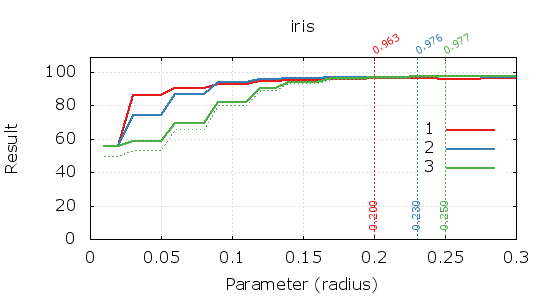
\includegraphics[width=.75\textwidth]{plots/experiment_6_iris.png}
	\captionof{figure}{Ensemble of one-, two- and threedimensional \emph{exposers}.}
	\label{fig:experiment_6}
}\end{experiment}